\documentclass[border=5pt]{standalone}
\usepackage{helvet}
\renewcommand{\familydefault}{\sfdefault}
\usepackage{tikz}
\usepackage{amsmath}
\usetikzlibrary{positioning,arrows.meta,fit,backgrounds,calc}

\begin{document}
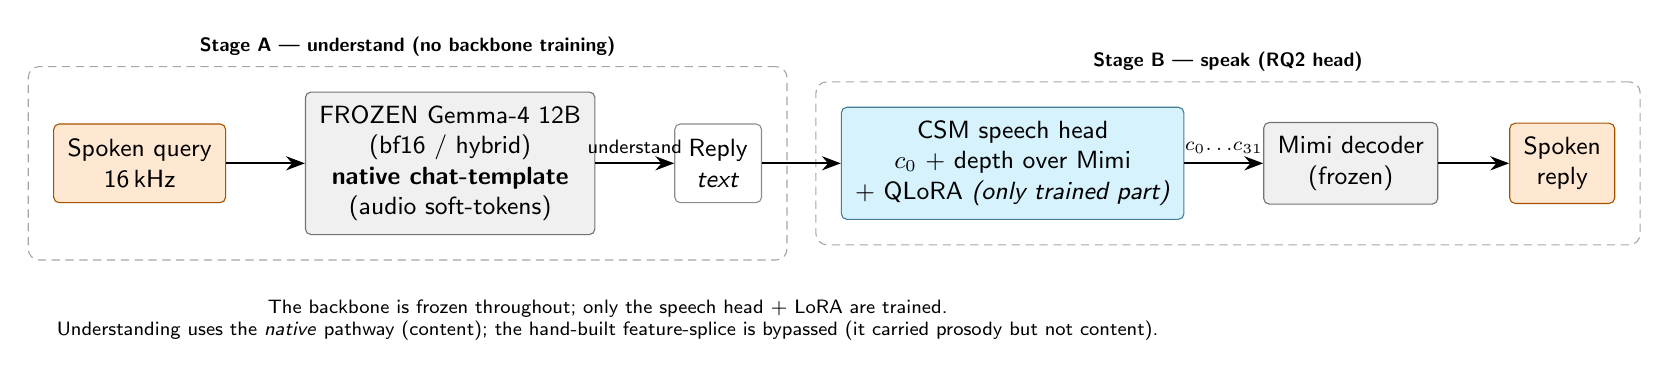
\begin{tikzpicture}[
  font=\small,
  box/.style={rectangle, rounded corners=2pt, draw=black!55, align=center,
              inner sep=5pt, minimum height=10mm},
  frozen/.style={box, fill=gray!12},
  trained/.style={box, fill=cyan!16, draw=cyan!55!black},
  io/.style={box, fill=orange!18, draw=orange!65!black, minimum height=10mm},
  txt/.style={box, fill=white, draw=black!45},
  arr/.style={-{Stealth[length=2.4mm]}, semithick},
  stage/.style={rectangle, rounded corners=4pt, draw=black!35, densely dashed,
                inner sep=9pt},
]

% ---- Stage A: understand ----
\node[io] (q) {Spoken query\\16\,kHz};
\node[frozen, right=10mm of q] (bb) {FROZEN Gemma-4 12B\\(bf16 / hybrid)\\\textbf{native chat-template}\\(audio soft-tokens)};
\node[txt, right=10mm of bb] (reply) {Reply\\\emph{text}};

\draw[arr] (q) -- (bb);
\draw[arr] (bb) -- node[above,font=\scriptsize]{understand} (reply);

% ---- Stage B: speak ----
\node[trained, right=10mm of reply] (head) {CSM speech head\\$c_0$ $+$ depth over Mimi\\$+$ QLoRA \emph{(only trained part)}};
\node[frozen, right=10mm of head] (mdec) {Mimi decoder\\(frozen)};
\node[io, right=9mm of mdec] (out) {Spoken\\reply};

\draw[arr] (reply) -- (head);
\draw[arr] (head) -- node[above,font=\scriptsize]{$c_0\!\dots\!c_{31}$} (mdec);
\draw[arr] (mdec) -- (out);

% ---- stage frames ----
\begin{scope}[on background layer]
  \node[stage, fit=(q)(bb)(reply), label={[font=\scriptsize\bfseries]above:Stage A --- understand (no backbone training)}] {};
  \node[stage, fit=(head)(mdec)(out), label={[font=\scriptsize\bfseries]above:Stage B --- speak (RQ2 head)}] {};
\end{scope}

% ---- note ----
\node[font=\scriptsize, align=center, below=7mm of bb.south, xshift=20mm] (note)
  {The backbone is frozen throughout; only the speech head $+$ LoRA are trained.\\
   Understanding uses the \emph{native} pathway (content); the hand-built
   feature-splice is bypassed (it carried prosody but not content).};

\end{tikzpicture}
\end{document}
